% options:
% thesis=B bachelor's thesis
% thesis=M master's thesis
% czech thesis in Czech language
% slovak thesis in Slovak language
% english thesis in English language
% hidelinks remove colour boxes around hyperlinks
% 10pt 11pt 12pt

\documentclass[thesis=M,slovak]{FITthesis}[2013/05/06]

\usepackage[utf8]{inputenc} % LaTeX source encoded as UTF-8

\usepackage{graphicx} %graphics files inclusion
\usepackage{hyperref} %hypertext
\usepackage{listings}
\lstset{language=Python,
breakatwhitespace=false,         % sets if automatic breaks should only happen at whitespace
  breaklines=true,                 % sets automatic line breaking
} 
% \usepackage{amsmath} %advanced maths
% \usepackage{amssymb} %additional math symbols

\usepackage{dirtree} %directory tree visualisation

% % list of acronyms
% \usepackage[acronym,nonumberlist,toc,numberedsection=autolabel]{glossaries}
% \iflanguage{czech}{\renewcommand*{\acronymname}{Seznam pou{\v z}it{\' y}ch zkratek}}{}
% \makeglossaries

\newcommand{\tg}{\mathop{\mathrm{tg}}} %cesky tangens
\newcommand{\cotg}{\mathop{\mathrm{cotg}}} %cesky cotangens

% % % % % % % % % % % % % % % % % % % % % % % % % % % % % % 
% ODTIALTO DALEJ VSETKO ZMENTE
% % % % % % % % % % % % % % % % % % % % % % % % % % % % % % 

\department{Katedra softwarového inženýrství}
\title{Spracovanie a vizualizácia chemických meraní v dátovom repozitári}
\authorGN{Lukáš} %(krstné) meno (mená) autora
\authorFN{Koštenský} % priezvisko autora
\authorWithDegrees{Bc. Lukáš Koštenský} %meno autora včetne súčasných akademických titulov
\supervisor{RNDr. David Antoš, Ph.D.}
\acknowledgements{Doplňte, ak chcete niekomu za niečo poďakovať. V~opačnom prípade úplne odstráňte tento príkaz.}
\abstractCS{V niekoľkých vetách zhrňte obsah a prínos tejto práce v~slovenčine. Po prečítaní abstraktu by mal čitateľ mať dosť informácií pre rozhodnutie, či Vašu prácu chce čítať.}
\abstractEN{Sem doplňte ekvivalent abstraktu Vašej práce v~angličtině.}
\placeForDeclarationOfAuthenticity{V~Prahe}
\declarationOfAuthenticityOption{1} %voľba Prehlásenia (číslo 1-6)
\keywordsCS{Nahraďte zoznamom kľúčových slov v slovenčine oddelených čiarkou.}
\keywordsEN{Nahraďte zoznamom kľúčových slov v angličtine oddelených čiarkou.}
% \website{http://site.example/thesis} %volitelná URL práce, objeví se v tiráži

\begin{document}

% \newacronym{CVUT}{{\v C}VUT}{{\v C}esk{\' e} vysok{\' e} u{\v c}en{\' i} technick{\' e} v Praze}
% \newacronym{FIT}{FIT}{Fakulta informa{\v c}n{\' i}ch technologi{\' i}}

\begin{introduction}
	%sem napíšte úvod Vašej práce
\end{introduction}

\chapter{Popis problému}
Repozitár slúži vo všeobecnosti ako centrálne miesto, ktoré sa stará o ukladanie a správu dát. Takúto službu môžu chcieť poskytovať rôzne inštitúcie, napríklad školy, knižnice,... Pod slovom repozitár si môžeme taktiež predstaviť konkrétny software, ktorý sa stará o ukladanie, archiváciu a sprístupnenie dát. V tejto diplomovej práci budeme pod slovom repozitár rozumieť práve software.

\section{Zdieľanie dát v tíme}
Ústav organickej chémie VŠCHT Praha potrebuje vyriešiť ukladanie a sprístupnenie dát. Potrebuje ukladať, analyzovať a prezentovať infračervené vibračné, NMR a hmotnostné spektroskopické merania, chemické vzorce a reakcie.

Nad jedným datasetom môže pracovať viacero ľudí, ktorí môžu riešiť rôzne merania a pokusy alebo spoločne pracovať na jednom meraní. V oboch prípadoch počas priebehu samotného výskumu potrebujú prístup k dátam, ktoré vytvoril iný člen tímu. Taktiež musia mať možnosť dáta upravovať (napr. opakované merania a pokusy, keď je potrebné doplniť nové výsledky). Repozitár teda musí umožniť zdieľanie dát v tíme, rôzne oprávnenia pre osoby, ktoré majú mať k dátam prístup, verziovanie dát.

\section{Open data/Open access}
Pri vývoji repozitára je potrebné myslieť na možnosť zverejnenia (časti) dát pre širokú verejnosť s možnosťou ich ďalšieho využitia alebo odkazovania sa na ne. Takto zverejnené dáta označujeme pojmom Open data. V prípade zverejnených výskumov hovoríme o Open access (OA). Repozitár musí umožniť zverejnenie všetkých alebo časti uložených dát. Cieľom vývoja repozitára je vytvorenie platformy, s ktorej využitím bude možné publikovať nielen články a závery výskumu, ale aj čiastkové merania a experimenty, ktoré k výsledkom viedli.

\section{Zálohovanie a archivácia}
Zálohovaním dát rozumieme vytváranie kópie práve spracúvaných alebo v relatívne nedávnej dobe uložených dát. Archiváciou rozumieme uschovávanie dokumentačných materiálov.

Zálohované dáta môžu byť poškodené degradáciou média, fyzickým poškodením média alebo v súčasnosti rozšírenými cryptovírusmi. Zálohovať dáta na jedno médium nestačí. Je dobré sa riadiť pravidlom 3-2-1. Tri kópie všetkých dôležitých dát, na dvoch rôznych médiách, pričom jedna kópia by mala byť uložená off-site, teda niekde mimo pracovného prostredia. \cite{zalohovanie}

Pri archivácii dát je potrebné myslieť na čitateľnosť dát po dlhej dobe. Preto je potrebné myslieť nielen na zabezpečenie dát, ale aj na archiváciu programu potrebného na prečítanie archivovaných dát.

Repozitár by mal byť pre užívateľov možnosťou ako dáta zálohovať. Zároveň jeho napojenie na služby CESNETu umožní ochranu dát, akú by bolo na pracovisku VŠCHT Praha ťažké dosiahnuť.

V budúcnosti bude možné repozitár rozšíriť o nástroje, ktoré by umožnili aj dlhodobú archiváciu dát.

\chapter{Súčasné riešenia}
\section{Repozitáre}
Existujú rôzne repozitáre, ktoré sa od seba líšia použitou technológiou, možnosťou rozšírenia, používajú rôzne metadátové schémy. Niektoré sú voľne dostupné ako open source, iné ako proprietárny software alebo hosťované aplikácie. V tejto časti uvádzam prehľad dostupných aplikácií. Zameriavam sa najmä na vlastnosti, ktoré boli pre ďalší vývoj repozitára kľúčové, a to: open source (aby bolo možné software ďalej upravovať), použitie metadátovej schémy, modulárnosť softwaru (jednoduchá možnosť rozšírenia o ďalšie nástroje) a verziovanie (najmä kvôli zdieľaniu a zálohovaniu dát).

% Tento software sa zameriava na dokumenty, ktoré majú byť voľne dostupné (anglicky Open Access) a online. Najčastejšie sa do takýchto inštitucionálnych repozitárov ukladajú textové dokumenty, pre ktoré je software najlepšie prispôsobený.

\subsection{Metadáta}
Na popis uložených dokumentov slúžia metadáta. Metadáta sú štrukturované dáta nesúce informáciu o primárnych dátach.\cite{iso8459-5} Kvôli vzájomnej prepojenosti repozitárov, vyhľadávaniu dát a správnej interpretácii informácií je snaha o~vyvinutie celosvetovo používaného štandardu pre popis dát.

O to sa snažia rôzne metadátove schémy, pomocou ktorých je možné zdroje popísať. Medzi najznámejšie schémy patrí Dublin Core [\url{http://dublincore.org/}] a MARC [\url{http://www.loc.gov/marc/}].

\subsubsection{Dublin Core}
Dublin Core (skrátene DC) vznikol s cieľom jednoducho a všeobecne popísať webové zdroje. Táto schéma obsahuje 15  prvkov. To sú: názov (title), autor (creator), predmet (subject), popis (description), vydavateľ (publisher), prispievateľ (contributor), dátum (date), typ (type), formát (format), identifikátor (identifier), zdroj (source), jazyk (language), vzťah (relation), pokrytie (coverage) a práva (rights). Tieto prvky nie sú povinné a môžu sa opakovať. Jednotlivé vlastnosti sú teda pomenované. Ako sa World Wide Web menil, v snahe o vytvorenie sémantického webu, vyvinul sa aj štandard Dublin Core. Od roku 2008 obsahuje formálne domény a rozsahy v definíciách vlastností. Tento aktualizovaný variant vlastností sa nazýva dcterms. Jednotlivé prvky môžu byť ďalej rozšírené o kvalifikátor. Ten môže lepšie určiť, čo daná položka popisuje. Napríklad namiesto všeobecného autora tak môžeme upresniť, či išlo o ilustrátora (dc:creator.ilustrator), editora (dc:creator.editor),...  Pre systémy, ktoré kvalifikátory nepoužívajú, ale musí zostať význam zachovaný.

\subsubsection{MARC}
MARC využívajú najmä knihovníci. Bol navrhnutý pre popis bibliografických údajov v strojovo čitateľnej podobe.
Schéma obsahuje vlastnosti, ktoré sú očíslované. Kým názov v dcterms je označený ako title, v MARCu  je označený číslom 245 (title proper statement). Na rozdiel od dcterms obsahuje niekoľko pomocných polí (ako napríklad 222 kľúčový názov, 240 unifikovaný názov,...). Takéto označenie je ľahko čitateľné pre stroje, knihovníci si pri každodennej práci s týmito číslami, ich významy zapamätajú. Človek, ktorý ich vidí prvýkrát, významu nerozumie.

MARC je od DC komplikovanejší, dokáže však presnejšie popísať zdroj.
Prvé číslo v číselných kódoch určuje, o aký typ informácie ide, jednotlivé kódy sú popísané v tabuľke \ref{tab:marc}. V prípade kódov 1XX, 4XX, 6XX, 7XX a 8XX sa obsah upresňuje doplnením dvojice čísel. Zvyčajne sa dodržiavajú nasledujúce dvojice: X00 - Mená osôb, X40 - Bibliografické názvy, X10 - Názvy firiem, X50 - Tematické pojmy, X11 - Názvy stretnutí/konferencií, X51 - Názvy miest, X30 - Jednotné názvy.

\begin{table}\centering
 	\caption[MARC]{Typ informácie v kóde MARC}\label{tab:marc}
 	\begin{tabular}{|l|l|c|c|}\hline
0XX	& Kontrolná informácia, identifikačné a klasifikačné čísla,...\tabularnewline \hline
1XX	& Hlavné údaje \tabularnewline \hline
2XX	& Názvy a kapitoly (názov, edícia, vydanie) \tabularnewline \hline
3XX	& Fyzický popis,... \tabularnewline \hline
4XX	& Informácie o dieloch/sériách \tabularnewline \hline
5XX	& Poznámky \tabularnewline \hline
6XX	& Kontaktné informácie na subjekty \tabularnewline \hline
7XX	& Pridané informácie (iné než o subjektoch, dieloch/sériách); linkovacie polia \tabularnewline \hline
8XX	& Rada pridaných informácií, informácie o holdingoch \tabularnewline \hline
9XX	& Vyhradené pre lokálnu implementáciu \tabularnewline \hline
 	\end{tabular}
 \end{table}


Použitie navrhovaného repozitára by malo byť jednoduché aj pre užívateľov, ktorí s metadátami nemajú veľké skúsenosti a nepotrebujú komplikovaný popis dát. Pre skúsenejších užívateľov by však bolo dobré zachovať možnosť použitia zložitejších, prípadne vlastných metadátových schém. Repozitár by teda mal vedieť používať aj iné metadátove schémy než len Dublin Core alebo MARC.

\subsection{Software}
V tejto časti popisujem prehľad najrozšírenejších softwarov, ktoré sa používajú ako implementácie repozitárov. Uvádzam prehľad pre nás dôležitých vlastností a to, či ide o proprietárny alebo open source systém, kvôli možnosti ďalších úprav; programovací jazyk a modulárnosť softwaru; aké metadátové schémy používajú a či ich je možné rozširovať; a či daný software umožňuje verziovanie uložených dát.

Pretože každý software pokrýva inú kombináciu týchto vlastností, repozitáre neklasifikujem, len uvádzam prehľad ich vlastností:

\subsubsection {Digital Commons}  [\url{http://digitalcommons.bepress.com/}]

Hostovaná platforma inštitucionálneho repozitára. Zameraný na školy a školské dokumenty.

Používa Dublin Core schému, v používateľskom rozhraní podporuje aj iné vlastnosti než len DC, aj keď nepodporuje iné schémy (vrátane MARC).

Autori vedia prispôsobiť repozitár požiadavkám klienta.

Nepodporuje verziovanie.

\subsubsection {LIBSYS}  [\url{http://www.libsys.co.in/}]

Proprietárny software. Repozitár funguje ako webová aplikácia.

Používa MARC ako schému metadát.

\subsubsection {SimpleDL}  [\url{http://www.simpledl.com/}]

Proprietárny software.

Metadáta na základe Dublin Core. Môžu byť rozšírené o iné schémy.

\subsubsection {Greenstone}  [\url{http://www.greenstone.org/}]

Repozitár vyvinutý na Univerzite Waikato.

Používa MARC schému.

Modulárna architektúra, napísaný v jazyku Java. Pluginy v jazyku Perl.

Nepodporuje verziovanie.

Open source

\subsubsection {Invenio}  [\url{http://inveniosoftware.org/}]

Software bol pôvodne vyvinutý pre CERN. Umožňuje vytvoriť digitálnu knižnicu alebo repozitár dokumentov dostupný cez web. 

Používa špecifikáciu MARC pre metadáta.

Má modulárnu architektúru. Napísaný v jazyku Python.

Podporuje verziovanie uložených dát.

Open Source

%\subsubsection {Zenodo} [\url{https://zenodo.org/}]
%
%Vyvinutý na základe Invenia, taktiež pre CERN. Má teda rovnaké vlastnosti ako Invenio.

\subsubsection {EPrints} [\url{http://www.eprints.org/}]

Vyvinutý na Univerzite Southampton.

Používa rôzne typy metadátových polí, ktoré je možné nastavovať (upraviť zobrazovanie, indexovanie, vyhľadávanie).

Modulárny software napísaný v jazyku Perl.

Podporuje verziovanie dát.

Open Source

\subsubsection {DSpace} [\url{http://www.dspace.org/}]

Software pôvodne vyvinutý MIT a Hewlett-Packard. Od vzniku má viac ako 2000 inštalácií po celom svete. 

Ako východziu schému pre popis dát používa Dublin Core, je však možné použiť aj iné schémy.

Ide o súbor spolupracujúcich Java webových aplikácií. K dispozícií je RESTful webové užívateľské rozhranie.

Neumožňuje verziovanie uložených dát.

Open source

\subsubsection {Fedora} [\url{http://www.fedora-commons.org/}]

Je možné použiť rôzne schémy pre popis dát.

Flexibilný, jednoducho rozšíriteľný, modulárny repozitár. Napísaný v programovacom jazyku Java.

Umožňuje verziovanie uložených dát.

Open Source


\section{Nástroje na zber a organizáciu chemických dát}
Výskumníci v oblasti chémie si vedú laboratórne denníky so záznamami hypotéz, experimentov, analýz alebo interpretáciou experimentov. V súčasnosti sa denníky vedú v elektronickej forme s využitím elektronických laboratórnych denníkov (často sa pre tento software používa skratka ELN). Pretože Ústav organickej chémie VŠCHT Praha používa a naďalej chce používať len E-Notebook a Open Enventory, iné nástroje na zber a organizáciu chemických dát v prehľade neuvádzam.

Prehľad programov, ktoré používa Ústav organickej chémie VŠCHT Praha:
\subsection{E-Notebook} [\url{http://www.cambridgesoft.com/Ensemble/E-notebook/}]
Software od firmy Perkin Elmer. V súčasnosti je k dispozícii len ako Enterprise verzia s inštaláciou na serveroch Oracle priamo pre koncového zákazníka alebo ako súčasť cloudových aplikácií Elements \url{https://elements.perkinelmer.com/} a plánovaného ChemDraw E-notebook \url{http://chemdrawenotebook.perkinelmer.cloud/}.

\subsection{Open Enventory} [\url{https://www.chemie.uni-kl.de/goossen/open-enventory/}]
Webová open source aplikácia napísaná v jazyku PHP. Využíva MySQL databázu.


% v rámci diplomovej práce pracujem s Fedorou verzie 4.5.
% Kvôli požiadavkom, ktoré sú kladené na repozitár, budeme potrebovať upraviť fungovanie REST frameworku. A to tak, aby aplikácia kontrolovala oprávnenia na zmenu stavov už pri spracovaní požiadavku.

% Nad RESTapi bude postavené užívateľské webové rozhranie. Napájať sa teda budeme na vrstvu, ktorá sa stará o prístup k dátam a ich uchovávanie.

%\begin{figure}[h]
%\centering
%\caption{Architektúra komponentov \url{https://wiki.duraspace.org/display/FEDORA45/Fedora+4.5+Documentation}}
%\includegraphics[width=1.0\textwidth]{f4-stack.jpg}
%\end{figure}
%
%
%\begin{figure}[h]
%\centering
%\caption{Integrácia komponentov \url{https://wiki.duraspace.org/display/FEDORA45/Fedora+4.5+Documentation}}
%\includegraphics[width=1.0\textwidth]{f4-arch.png}
%\end{figure}
%
%
%Systémove požiadavky:
%\begin{enumerate}
%	\item Java 8
%	\item Servlet 3.0 container (Tomcat 7 a novší, Jetty 9.x a novší...)
%\end{enumerate}

\chapter{Analýza a návrh riešenia}
\section{Analýza požiadaviek}
\subsection{Funkčné požiadavky}
Repozitár musí umožniť:
\begin{itemize}
	\item Uložiť nové dáta.
	\item Upraviť existujúce dáta.
	\item Zobraziť existujúce dáta.
	\item Uložiť históriu zmien dát.
	\item Vyhľadávať v metadátach.
	\item Import dát z aplikácie Open Eventory.
\end{itemize}

Prístup k jednotlivým objektom a poliam ale môže byť limitovaný. Vytváranie a úprava jednotlivých objektov je umožnená len konkrétnym užívateľom.

Aplikácia Open Eventory musí byť upravená tak, aby umožnila export dát vo formáte vhodnom pre import do repozitára.

\subsection{Požiadavky na vlastnosti repozitára}
\begin{itemize}
	\item Repozitár bude pre užívateľov dostupný ako webová aplikácia.
	\item Repozitár musí umožniť ďalšie rozšírenie pre iné typy dát.
	\item Repozitár bude napojený na služby CESNETu.
\end{itemize}

\section{Výber technológií}
\subsection{Fedora}
Keďže ani jeden existujúci repozitár nespĺňa všetky požiadavky alebo nevie uložiť/zobraziť dáta pre Ústav organickej chémie VŠCHT Praha, bolo potrebné vytvoriť nový alebo upraviť stávajúci software. Vytvorenie nového softwaru od základov by bolo neefektívne. Vyššie zmienené repozitáre fungujú, niektoré ich časti by teda boli programované nanovo. Zvolená bola možnosť doplniť/upraviť funkčnosť existujúceho repozitára. Výber vhodného repozitára bol možný z open source repozitárov, ktoré umožňujú úpravu kódu.

Okrem toho boli pri výbere vhodného repozitára do úvahy brané ďalšie kritériá. A to možnosť použitia viacerých metadátových schém, programovací jazyk, podpora komunity. Do finálneho výberu sa dostali DSpace a Fedora. Oba repozitáre sú podobne výkonné (zvládajú milióny záznamov).

Vďaka návrhu Fedory je do tohto softwaru jednoduchšie pridávanie rozšírení, taktiež už má vyriešené verziovanie uložených dát. DSpace má k dispozícii webové užívateľské rozhranie, ktoré je možné upravovať a ďalej rozširovať. Fedora používa jednoduché webové rozhranie, ktoré umožňuje len základnú prácu s dátami. Vytvorenie samostatného, nového webového užívateľského rozhrania s využitím RESTapi je ale jednoduchšie než úprava jadra DSpace, aby zvládal verziovanie uložených dát.

Z existujúcich možností bola zvolená Fedora ako najvhodnejší software pre možnosť ďalších potrebných úprav pre použitie v rámci služieb CESNET z.s.p.o. a splnenie požiadaviek Ústavu organickej chémie VŠCHT Praha.

\subsection{Elasticsearch}
Na vyhľadávanie v repozitári bude použitá samostatná aplikácia Elasticsearch \url{https://www.elastic.co/products/elasticsearch}. Aplikácia umožňuje veľmi rýchle vyhľadávanie v indexovaných dátach. Dopyty je možné posielať s využitím RESTful api a JSONu.


\chapter{Implementácia}
\section{Návrh aplikácie}
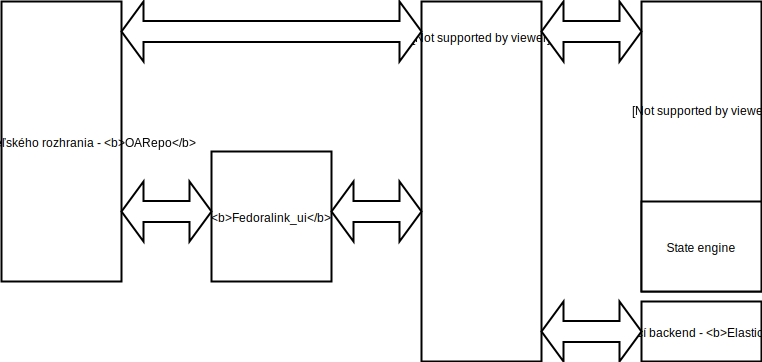
\includegraphics[width=1.0\textwidth]{diagramy/Architektura_repozitara.pdf}

\subsection{Fedora}
Ako už bolo zmienené v predchádzajúcej kapitole, ako backend pre repozitár bola zvolená Fedora. V nej sú uložené dáta, metadáta, typy modelov spolu s HTML šablónami, stavy a oprávnenia (ACL).

Metadáta vo Fedore sú uložené vo formáte RDF (Resource Description Format), teda ako trojice - subjekt, predikát a objekt.

\subsection{State engine}
Pre možnosť využívania stavov bude nutné rozšíriť Fedoru o tento modul. Modul rieši prechody medzi stavmi, zmenu stavov, zmenu kontroléru stavov, konkrétnu operáciu povolí len oprávneným osobám. Oprávnené osoby sú určené pomocou ACL.

\subsection{Fedora\_group\_plugin}
Doplňujúci modul do Fedory, ktorý umožňuje overenie oprávnení aj na základe členstva v django skupinách. Samotná Fedora s webac umožňuje overenie autorizácie na základe štandardnej On-Behalf-Of hlavičky, o ktoré sa stará DelegateHeaderPrincipalProvider. Rozšírenie Fedora\_group\_plugin umožňuje autorizáciu na základe On-Behalf-Of-Django-Groups hlavičky, o ktoré sa stará DjangoGroupPrincipalProvider. Autorom tohto pluginu je Mgr. Miroslav Šimek. 

Plugin je súčasťou git repozitára fedoralinku. Impersonifikácia na iného užívateľa alebo skupinu je umožnená len pod FedoraAdmin užívateľom. Hodnota posielaná v týchto hlavičkách je vo forme urn.
Ak teda máme na vstupe užívateľské meno vo forme emailu (napr. \uv{user@vscht.cz}), výsledná hodnota bude \uv{urn:vscht.cz:user}, inak je v tvare \uv{urn:user}. 
Skupiny sú získané z užívateľovych skupín v Djangu.

Vďaka tomuto rozšíreniu bude možné jednoduché rozšírenie repozitára o autentizáciu cez iného poskytovateľa identity (napr. Shibboleth).

\subsection{Elasticsearch}
Aplikácia, ktorá umožňuje rýchle vyhľadavánie v metadátach.

\subsection{Fedoralink}
Aplikácia napísaná pre potreby repozitára záverečných prác VŠCHT Praha, v programovacom jazyku Python s využitím frameworku Django, stará sa o komunikáciu s Fedorou a Elasticsearch. Autorom fedoralinku je Mgr. Miroslav Šimek. Fedoralink bol počas vývoja repozitára ďalej upravovaný v rámci diplomovej práce. Aktuálnu verziu je možné nájsť na \url{https://github.com/CESNET/fedoralink}

\subsubsection{FedoraObject}
Aby bolo možné z objektami získanými z Fedory pracovať ako s objektami v Djangu, boli vytvorené triedy, ktoré s týmito objektami pracujú. Trieda FedoraObject je základnou triedou pre tieto objekty. S dátami získanými vo formáte RDF z Fedory umožňuje pracovať aj keď vopred nepoznáme štruktúru týchto dát.

Ak potrebujeme získať alebo upraviť niektorú metadátovú položku pracujeme s objektom následovne (v tomto prípade chceme získať alebo upraviť názov - title zo schémy Dublin Core) : 
\begin{lstlisting}[frame=single] 
# [RDF:Name]
obj[DC.title]
\end{lstlisting}

Z objektu môžeme získať jeho ID, URL identifikátor (slug), jeho potomkov, objekt uložiť späť do Fedory alebo ho zmazať.

Objekt vo Fedore môže byť typu container alebo bitstream. V druhom prípade môže mať k sebe priradený súbor. Preto aj táto trieda FedoraObject umožňuje prácu so získaným bitstreamom a to pomocou funkcie get\_bitstream.

\subsubsection{IndexableFedoraObject}
Rozširuje triedu FedoraObject. Ak využívame túto triedu, o schéme metadát musíme vedieť ďalšie informácie. Vieme akého typu sú jednotlivé metadátové polia (napr. či ide o reťazec, pole, ktoré môže byť vo viacerých jazykoch alebo o dátum...).

Príklad využitia IndexableFedoraObject:
\begin{lstlisting}[frame=single] 
#
# DCObject is indexable and provides .title and .creator property, that get mapped to
# DC.* predicates in RDF by simple_namespace_mapper
#
class DCObject(IndexableFedoraObject):

    title         = IndexedLanguageField(DC.title, required=True,
                                         verbose_name=_('Title'))

    alternative   = IndexedTextField(DC.alternative,
                                     verbose_name=_('Alternative title'))

    abstract      = IndexedLanguageField(DC.abstract,
                                         verbose_name=_('Abstract'),
                                         attrs={'presentation': 'textarea'})

    creator       = IndexedTextField(DC.creator,
                                     verbose_name=_('Creator'))

    contributor   = IndexedTextField(DC.contributor,
                                     verbose_name=_('Contributor'))

    dateSubmitted = IndexedDateTimeField(DC.dateSubmitted,
                                         verbose_name=_('Date submitted'))

    dateAvailable = IndexedDateTimeField(DC.dateAvailable,
                                         verbose_name=_('Date available'))

    class Meta:
        rdf_types = (DC.Object,)
\end{lstlisting}

Trieda DCObject bude využitá pri dátach získaných z Fedory, ktoré obsahujú metadáta podľa schémy DublinCore. Samotná trieda dedí z triedy IndexableFedoraObject.

IndexedLanguageField - metadátové pole, ktoré môže byť vo viacerých jazykoch. Za samotnou hodnotov je vložený parameter \uv{@lang}, ktorý podľa skratky jazyka (\uv{en}, \uv{cs}) určuje, v akom jazyku je daná hodnota.
IndexedTextField - metadátové pole, ktoré obsahuje textový reťazec.
IndexedDateTimeField - metadátové pole obsahujúce dátum a čas.

RDF typ je taktiež uložený vo Fedore a umožnuje mapovať získaný objekt na správnu triedu.

\subsubsection{FedoraTypeManager}
Trieda (singleton) zodpovedná za vytvorenie inštancie FedoraObject (alebo jej podtriedy) podľa RDF metadát získaných z Fedory počas behu aplikácie. Objekt získaný z Fedory môže mať viacero RDF typov a teda spadať do viacero tried. Z nich sa vyberie najvhodnejšia alebo sa pomocou viacnásobnej dedičnosti vytvorí nová trieda kombinujúca vlastnosti viacerých existujúcich tried,  ktorá sa následne použije pre prácu s takto získaným objektom z Fedory.

Získanie správnej triedy pre objekt má na starosť funkcia get\_object\_class:
\begin{lstlisting}[frame=single] 
@staticmethod
def get_object_class(metadata, model_class=None):
   """
   Returns the best python class for the given metadata

   :param metadata:    the metadata
   :return:            python class which fits the metadata
   """

   from .models import FedoraObject

   types = metadata[RDF.type]

   possible_classes = {FedoraObject: 0}
   if model_class:
        possible_classes[model_class] = 1

   # look at classes registered on rdf types and if the class match, add it to the dict of possible classes
    for clz, rdf_and_priority in FedoraTypeManager.on_rdf_types.items():
        if _type_matches(types, rdf_and_priority[0]):
            possible_classes[clz] = max(possible_classes.get(clz, 0), rdf_and_priority[1])

    # look at classes registered on rdf predicates and if the class match, add it to the dict of possible classes
    for clz, rdf_and_priority in FedoraTypeManager.on_rdf_predicates.items():
         if _has_predicates(metadata, rdf_and_priority[0]):
             possible_classes[clz] = max(possible_classes.get(clz, 0), rdf_and_priority[1])

    # call class method handles_metadata and if it returns a priority, add the class as well
    for clz in FedoraTypeManager.models:
         priority = getattr(clz, 'handles_metadata')(metadata)
         if priority is not None and priority >= 0:
             possible_classes[clz] = max(possible_classes.get(clz, 0), priority)

    # convert to a list, add priorities from superclasses as well
    # (i.e. 2 * current_priority + sum of priorities of superclasses)
    propagated_possible_classes = []

    for clazz, priority in possible_classes.items():

        for clz in inspect.getmro(clazz):
            if clz in possible_classes:
                priority += possible_classes[clz]

        propagated_possible_classes.append((clazz, priority))

    # sort by priority
    propagated_possible_classes.sort(key=lambda x: -x[1])

    # remove classes that are in mro of other classes
    classes = []
    seen_classes = set()
    for clazz, priority in propagated_possible_classes:
        if clazz in seen_classes:
           continue

        classes.append(clazz)

        for clz in inspect.getmro(clazz):
            seen_classes.add(clz)

    # got a list of classes, create a new type (or use a cached one ...)
    return FedoraTypeManager.generate_class(classes)
\end{lstlisting}



\subsection{Fedoralink\_ui}
Je súčasťou git repozitára fedoralinku. Modul sa stará o užívateľské rozhranie aplikácie. Pre komunikáciu s Fedorou využíva fedoralink.

\subsubsection{Mapovanie generických URL adries}
Funkcie v rámci súboru {\em generic\_urls.py} mapujú URL adresy v aplikácii na správne časti kódu pre zobrazenie, editáciu alebo vyhľadávanie. Z URL adresy zistíme ID objektu alebo kolekcie vo Fedore.

Vzory využívajúce regulárne výrazy pre URL adresy:
\begin{itemize}
	\item '\textasciicircum\$' - index
	\item r'\textasciicircum(?P<collection\_id>[a-fA-F0-9\_/-]*)?search(?P<parameters>.*)\$' - vyhľadávanie v rámci kolekcie
	\item '\textasciicircum(?P<id>.*)/addSubcollection\$' - pridanie novej subkolekcie
	\item '\textasciicircum(?P<id>.*)/add\$' - vytvorenie nového objektu ako potomka objektu s daným ID
	\item '\textasciicircum(?P<id>.*)/edit\$' - upravenie objektu s daným ID
	\item '\textasciicircum(?P<id>.*)\$' - zobrazenie objektu s daným ID
\end{itemize}

Tieto generické URL adresy môžu byť ďalej rozšírené v niektorej časti aplikácie.

\subsubsection{Získanie šablóny pre zobrazenie, editáciu objektu alebo zoznam objektov v kolekcii}
O zobrazenie správnych údajov v správnej šablóne, prípadne o vytvorenie nového objektu/kolekcie so správnymi údajmi sa ďalej stará kód v súbore views.py.

V samotnej aplikácii (vo fedoralinku alebo v koncovej aplikácii) musí byť model objektu - trieda v Pythone. Ostatné potrebné veci sú uložené priamo vo Fedore. V nej sú uložené jednotlivé typy objektov, pri kolekciách je uložený typ subkolekcií a potomkov. Tieto objekty môžu mať naviac uložené šablóny pre zobrazenie, úpravu a vytvorenie potomkov. Taktiež je možné do Fedory uložiť typy jednotlivých polí a k nim šablóny pre ich zobrazenie/editáciu.

Trieda ResourceType, ktorá dedí z IndexableFedoraObject umožňuje uložiť šablóny pre rôzne objekty. Získanie správneho typu objektu je možné vďaka párovaniu cez RDF typ.
\begin{lstlisting}[frame=single] 
class ResourceType(IndexableFedoraObject):
    label = IndexedTextField(CESNET_TYPE.label, verbose_name=_('Label'), level=IndexedField.MANDATORY)

    template_view = IndexedLinkedField(CESNET_TYPE.template_view, Template, verbose_name=_('Template for view'))

    template_edit = IndexedLinkedField(CESNET_TYPE.template_edit, Template, verbose_name=_('Template for edit'))

    template_list_item = IndexedLinkedField(CESNET_TYPE.template_list_item, Template,
                                            verbose_name=_('Template for item list view'))

    controller = IndexedTextField(CESNET_TYPE.controller, verbose_name=_('Controller class'),
                                  level=IndexedField.MANDATORY)

    rdf_types = IndexedTextField(CESNET_TYPE.rdf_types, verbose_name=_('RDF types'), level=IndexedField.MANDATORY,
                                 multi_valued=True)

    fedoralink_model = IndexedTextField(CESNET_TYPE.fedoralink_model, verbose_name=_('Fedoralink model class name'),
                                        level=IndexedField.MANDATORY)

    class Meta:
        rdf_types = (CESNET_TYPE.ResourceType,)
\end{lstlisting}

Kód vo views.py teda z ID získa objekt, ku ktorému nájde vo Fedore uložený správny typ. Z neho následne získa šablónu, ktorú zobrazí. Ak sa správna šablóna pre objekt alebo pole nenachádza vo Fedore, skúsi ju nájsť v aplikácii alebo použije všeobecné šablóny uložené vo fedoralink\_ui, ktoré umožňujú aspoň základné zobrazenie informácií.

\subsubsection{Cachovanie šablón}
Fedoralink\_ui taktiež obsahuje kód potrebný pre cachovanie výsledných šablón zložených zo šablón typu objektu a jednotlivých polí, keďže získanie týchto údajov z Fedory je časovo náročné. Pre získanie výslednej šablóny je potrebné množstvo dopytov na Elasticsearch a následne na Fedoru, počet dopytov záleží hlavne na komplikovanosti modelu objektu.

O cachovanie sa stará trieda {\em FedoraTemplateCache}.

Prehľad vybraných metód v triede:
\begin{lstlisting}[frame=single] 
@staticmethod
    def get_resource_type(rdf_meta):
        for rdf_type in rdf_meta:
            retrieved_type = list(ResourceType.objects.filter(rdf_types__exact=rdf_type))
            if retrieved_type:
                return retrieved_type[0]
        return None
\end{lstlisting}
Metóda {\em get\_resource\_type} umožňuje získať správny RDF typ objektu.

\begin{lstlisting}[frame=single] 
@staticmethod
@simple_cache
def _get_template_string_internal(rdf_types, view_type):
    return FedoraTemplateCache._load_template(FedoraTemplateCache.get_template_object(rdf_types, view_type))

@staticmethod
def _load_template(template_object):
    if template_object is not None and template_object.get_bitstream() is not None:
        return template_object.get_bitstream().stream.read().decode("utf-8")
    return None
\end{lstlisting}
Metóda {\em \_load\_template} získa bitstream z objektu šablóny, ktorý máme z Fedory. Bitstream následne dekóduje a uloží ako reťazec, dáta do Fedory ukladáme v kódovaní \mbox{utf-8}. O cachovanie tejto šablóny sa stará metóda {\em \_get\_template\_string\_internal}.

Repozitár záverečných prác VŠCHT Praha pôvodne využíval šablóny uložené priamo v kóde aplikácie. Po vzniku fedoralink\_ui ale aj tento repozitár začal využívať fedoralink\_ui.

\subsection{Návrh grafického rozhrania}
Repozitár bude nasadený ako jedna zo služieb diskového úložiska CESNET, z.s.p.o. \url{https://du.cesnet.cz/}, preto navrhnuté grafické rozhranie vychádza z už existujúcich služieb.

Návrh zobrazenia pre dáta organickej chémie:
\begin{figure}\centering
	\includegraphics[width=1.0\textwidth]{grafika/list_InfraredSpectra.png}
 	\caption[Výpis dát v kolekcii InfraredSpectra]{Výpis dát v kolekcii Infrared Spectra}\label{graphics:listInfrared}
\end{figure}

\begin{figure}\centering
	\includegraphics[width=1.0\textwidth]{grafika/detail_Ethanol.png}
 	\caption[Zobrazenie detailu konkrétnej položky (Ethanolu)]{Zobrazenie detailu konkrétnej položky (Ethanolu)}\label{graphics:Ethanol}
\end{figure}

\section{Automatický import dát}
Aby sme čo najviac zjednodušili vkladanie nových dát do repozitára, je potrebné upraviť niektorý z nástrojov na zber a organizáciu chemických dát, ktorý používajú výskumníci z Ústavu organickej chémie VŠCHT Praha. Pre účely diplomovej práce bol po dohode s výskumníkmi ako zdroj dát pre import vybraný nástroj Open Enventory.

K importu dát má dôjsť po kliknutí na tlačítko umiestnené priamo v tejto webovej aplikácii. Aby bolo možné aplikáciu upraviť, je potrebné vedieť ako funguje, aké sú vzťahy medzi tabuľkami v databázi a nájsť vhodné umiestnenie pre tlačítko.
Open Enventory je open source aplikácia, ktorá má k dispozícii všetky zdrojové kódy. Neexistuje k nej ale žiadna dokumentácia.

Pri prechádzaní kódu aplikácie som naviac zistil, že veľká časť komentárov a aj časť samotného kódu sú napísané v nemčine. Databázová schéma taktiež nie je prehľadná, v jednotlivých tabuľkách nie sú označené cudzie kľúče a teda chýbajú prepojenia na iné tabuľky. Na stĺpcoch, ktoré by mali byť cudzími kľúčami sú len indexy.

\subsection{Schéma databáze}
Celá schéma databáze je na priloženom CD vo formáte UML aj SVG. V tejto časti sú popísané a okomentované databázové tabuľky, v ktorých sú uložené dáta, ktoré chceme importovať do repozitára alebo ich k tomuto importu potrebujeme.

\begin{figure}\centering
	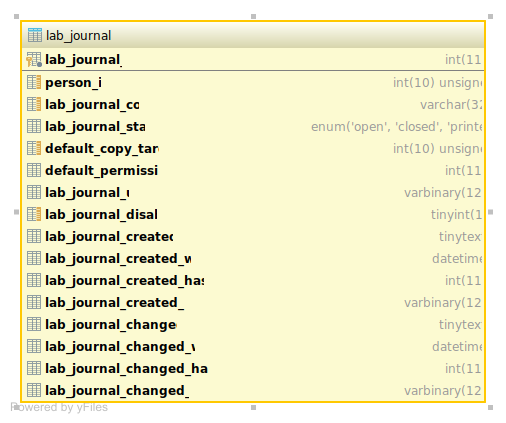
\includegraphics[width=1.0\textwidth]{Schema_DB_Open_Enventory/lab_journal.png}
 	\caption[Štruktúra databázovej tabuľky lab\_journal]{Štruktúra databázovej tabuľky lab\_journal}\label{graphics:lab_journal}
\end{figure}

V databázovej tabuľke lab\_journal, ktorej štruktúra je na obrázku \ref{graphics:lab_journal} sú uložené základné údaje o laboratórnom denníku. Pre naše účely budú ďalej dôležité stĺpce person\_id a primárny kľúč lab\_journal\_id.


\begin{conclusion}
	%sem napíšte záver Vašej práce
\end{conclusion}

\bibliographystyle{csn690}
\bibliography{mybibliographyfile}

\appendix

\chapter{Zoznam použitých skratiek}
% \printglossaries
\begin{description}
	\item[ELN] Electronic lab notebook
	\item[GUI] Graphical user interface
	\item[XML] Extensible markup language
	\item[RDF] Resource Description Format
	\item[ACL] Access control list
	\item[UML] Unified Modeling Language
	\item[SVG] Scalable Vector Graphics
\end{description}


% % % % % % % % % % % % % % % % % % % % % % % % % % % % 
% % Tuto kapitolu z výsledné práce ODSTRAŇTE.
% % % % % % % % % % % % % % % % % % % % % % % % % % % % 
% 
% \chapter{Návod k~použití této šablony}
% 
% Tento dokument slouží jako základ pro napsání závěrečné práce na Fakultě informačních technologií ČVUT v~Praze.
% 
% \section{Výběr základu}
% 
% Vyberte si šablonu podle druhu práce (bakalářská, diplomová), jazyka (čeština, angličtina) a kódování (ASCII, \mbox{UTF-8}, \mbox{ISO-8859-2} neboli latin2 a nebo \mbox{Windows-1250}). 
% 
% V~české variantě naleznete šablony v~souborech pojmenovaných ve formátu práce\_kódování.tex. Typ může být:
% \begin{description}
% 	\item[BP] bakalářská práce,
% 	\item[DP] diplomová (magisterská) práce.
% \end{description}
% Kódování, ve kterém chcete psát, může být:
% \begin{description}
% 	\item[UTF-8] kódování Unicode,
% 	\item[ISO-8859-2] latin2,
% 	\item[Windows-1250] znaková sada 1250 Windows.
% \end{description}
% V~případě nejistoty ohledně kódování doporučujeme následující postup:
% \begin{enumerate}
% 	\item Otevřete šablony pro kódování UTF-8 v~editoru prostého textu, který chcete pro psaní práce použít -- pokud můžete texty s~diakritikou normálně přečíst, použijte tuto šablonu.
% 	\item V~opačném případě postupujte dále podle toho, jaký operační systém používáte:
% 	\begin{itemize}
% 		\item v~případě Windows použijte šablonu pro kódování \mbox{Windows-1250},
% 		\item jinak zkuste použít šablonu pro kódování \mbox{ISO-8859-2}.
% 	\end{itemize}
% \end{enumerate}
% 
% 
% V~anglické variantě jsou šablony pojmenované podle typu práce, možnosti jsou:
% \begin{description}
% 	\item[bachelors] bakalářská práce,
% 	\item[masters] diplomová (magisterská) práce.
% \end{description}
% 
% \section{Použití šablony}
% 
% Šablona je určena pro zpracování systémem \LaTeXe{}. Text je možné psát v~textovém editoru jako prostý text, lze však také využít specializovaný editor pro \LaTeX{}, např. Kile.
% 
% Pro získání tisknutelného výstupu z~takto vytvořeného souboru použijte příkaz \verb|pdflatex|, kterému předáte cestu k~souboru jako parametr. Vhodný editor pro \LaTeX{} toto udělá za Vás. \verb|pdfcslatex| ani \verb|cslatex| \emph{nebudou} s~těmito šablonami fungovat.
% 
% Více informací o~použití systému \LaTeX{} najdete např. v~\cite{wikilatex}.
% 
% \subsection{Typografie}
% 
% Při psaní dodržujte typografické konvence zvoleného jazyka. České \uv{uvozovky} zapisujte použitím příkazu \verb|\uv|, kterému v~parametru předáte text, jenž má být v~uvozovkách. Anglické otevírací uvozovky se v~\LaTeX{}u zadávají jako dva zpětné apostrofy, uzavírací uvozovky jako dva apostrofy. Často chybně uváděný symbol "{} (palce) nemá s~uvozovkami nic společného.
% 
% Dále je třeba zabránit zalomení řádky mezi některými slovy, v~češtině např. za jednopísmennými předložkami a spojkami (vyjma \uv{a}). To docílíte vložením pružné nezalomitelné mezery -- znakem \texttt{\textasciitilde}. V~tomto případě to není třeba dělat ručně, lze použít program \verb|vlna|.
% 
% Více o~typografii viz \cite{kobltypo}.
% 
% \subsection{Obrázky}
% 
% Pro umožnění vkládání obrázků je vhodné použít balíček \verb|graphicx|, samotné vložení se provede příkazem \verb|\includegraphics|. Takto je možné vkládat obrázky ve formátu PDF, PNG a JPEG jestliže používáte pdf\LaTeX{} nebo ve formátu EPS jestliže používáte \LaTeX{}. Doporučujeme preferovat vektorové obrázky před rastrovými (vyjma fotografií).
% 
% \subsubsection{Získání vhodného formátu}
% 
% Pro získání vektorových formátů PDF nebo EPS z~jiných lze použít některý z~vektorových grafických editorů. Pro převod rastrového obrázku na vektorový lze použít rasterizaci, kterou mnohé editory zvládají (např. Inkscape). Pro konverze lze použít též nástroje pro dávkové zpracování běžně dodávané s~\LaTeX{}em, např. \verb|epstopdf|.
% 
% \subsubsection{Plovoucí prostředí}
% 
% Příkazem \verb|\includegraphics| lze obrázky vkládat přímo, doporučujeme však použít plovoucí prostředí, konkrétně \verb|figure|. Například obrázek \ref{fig:float} byl vložen tímto způsobem. Vůbec přitom nevadí, když je obrázek umístěn jinde, než bylo původně zamýšleno -- je tomu tak hlavně kvůli dodržení typografických konvencí. Namísto vynucování konkrétní pozice obrázku doporučujeme používat odkazování z~textu (dvojice příkazů \verb|\label| a \verb|\ref|).
% 
% \begin{figure}\centering
% 	\includegraphics[width=0.5\textwidth, angle=30]{cvut-logo-bw}
% 	\caption[Příklad obrázku]{Ukázkový obrázek v~plovoucím prostředí}\label{fig:float}
% \end{figure}
% 
% \subsubsection{Verze obrázků}
% 
% % Gnuplot BW i barevně
% Může se hodit mít více verzí stejného obrázku, např. pro barevný či černobílý tisk a nebo pro prezentaci. S~pomocí některých nástrojů na generování grafiky je to snadné.
% 
% Máte-li například graf vytvořený v programu Gnuplot, můžete jeho černobílou variantu (viz obr. \ref{fig:gnuplot-bw}) vytvořit parametrem \verb|monochrome dashed| příkazu \verb|set term|. Barevnou variantu (viz obr. \ref{fig:gnuplot-col}) vhodnou na prezentace lze vytvořit parametrem \verb|colour solid|.
% 
% \begin{figure}\centering
% 	\includegraphics{gnuplot-bw}
% 	\caption{Černobílá varianta obrázku generovaného programem Gnuplot}\label{fig:gnuplot-bw}
% \end{figure}
% 
% \begin{figure}\centering
% 	\includegraphics{gnuplot-col}
% 	\caption{Barevná varianta obrázku generovaného programem Gnuplot}\label{fig:gnuplot-col}
% \end{figure}
% 
% 
% \subsection{Tabulky}
% 
% Tabulky lze zadávat různě, např. v~prostředí \verb|tabular|, avšak pro jejich vkládání platí to samé, co pro obrázky -- použijte plovoucí prostředí, v~tomto případě \verb|table|. Například tabulka \ref{tab:matematika} byla vložena tímto způsobem.
% 
% \begin{table}\centering
% 	\caption[Příklad tabulky]{Zadávání matematiky}\label{tab:matematika}
% 	\begin{tabular}{|l|l|c|c|}\hline
% 		Typ		& Prostředí		& \LaTeX{}ovská zkratka	& \TeX{}ovská zkratka	\tabularnewline \hline \hline
% 		Text		& \verb|math|		& \verb|\(...\)|	& \verb|$...$|		\tabularnewline \hline
% 		Displayed	& \verb|displaymath|	& \verb|\[...\]|	& \verb|$$...$$|	\tabularnewline \hline
% 	\end{tabular}
% \end{table}
% 
% % % % % % % % % % % % % % % % % % % % % % % % % % % % 

\chapter{Obsah priloženého CD}

%upravte podle skutecnosti

\begin{figure}
	\dirtree{%
		.1 readme.txt\DTcomment{stručný popis obsahu CD}.
		.1 exe\DTcomment{adresár so spustiteľnou formou implementácie}.
		.1 src.
		.2 impl\DTcomment{zdrojové kódy implementácie}.
		.2 thesis\DTcomment{zdrojová forma práce vo formáte \LaTeX{}}.
		.1 text\DTcomment{text práce}.
		.2 thesis.pdf\DTcomment{text práce vo formáte PDF}.
		.2 thesis.ps\DTcomment{text práce vo formáte PS}.
	}
\end{figure}

\end{document}
